\documentclass[slidestop,14pt]{beamer}

\title{Genome of the Netherlands}
\providecommand{\myConference}{Lab-J work discussion}
\providecommand{\myDate}{Wednesday, 8 June 2011}
\author{Martijn Vermaat}
\providecommand{\myGroup}{Leiden Genome Technology Center}
\providecommand{\myDepartment}{Department of Human Genetics}
\providecommand{\myCenter}{Center for Human and Clinical Genetics}
\providecommand{\lastRightLogo}{
  \raisebox{-0.1cm}{
    
\includegraphics[scale = 0.055]{lgtc_logo}
  }
}
\providecommand{\lastCenterLogo}{}

\usetheme{lumc}

\begin{document}

% This disables the \pause command, handy in the editing phase.
%\renewcommand{\pause}{}

% Make the title page.
\bodytemplate

%\frame{
%  \frametitle{Genome of the Netherlands}
%  \tableofcontents
%}

\section{Introduction}

\frame{
  \frametitle{Genome of the Netherlands}
  \tableofcontents[currentsection]
}

\begin{frame}
  \frametitle{Genome of the Netherlands}

  \vspace{\baselineskip}

  Ultra-sharp genetic group portrait of the Dutch

  \pause

  \vspace{\baselineskip}

  Consortium of
  \begin{itemize}
    \item UMCG
    \item LUMC
    \item Erasmus MC
    \item VUMC
    \item UMCU
  \end{itemize}
\end{frame}

\begin{frame}
  \frametitle{Goals}

  \vspace{\baselineskip}

  Medical:
  \begin{itemize}
    \item Enrich biobank data
    \item Construct a Dutch reference genome
    \item Identify rare variants
  \end{itemize}

  \vspace{\baselineskip}

  Scientific:
  \begin{itemize}
    \item Gain high-throughput sequencing experience
    \item Develop new scientific methods
  \end{itemize}
\end{frame}

\begin{frame}
  \frametitle{Setup}

  \vspace{\baselineskip}

  \begin{itemize}
    \item 250 trios of parents and adult child
    \item Sequencing in China (BGI)
    \item Analysis in the Netherlands
  \end{itemize}

  \vspace{\baselineskip}

  
\includegraphics[width=0.3\linewidth,transparent]{parents-girl.png}
  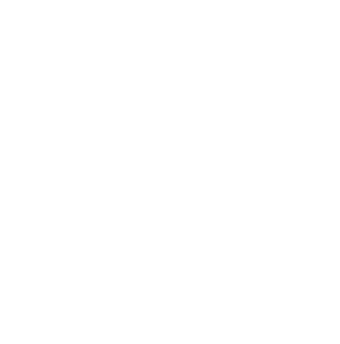
\includegraphics[width=0.3\linewidth,transparent]{parents-boy.png}
  
\includegraphics[width=0.3\linewidth,transparent]{parents-girl.png}
\end{frame}

\begin{frame}
  \frametitle{Sequencing method}

  \vspace{\baselineskip}

  \begin{itemize}
    \item Illumina HiSeq
    \item Full-genome
    \item 500M paired reads of 90b
    \item 12x average coverage
  \end{itemize}

  \vspace{0.5\baselineskip}

  \begin{center}
    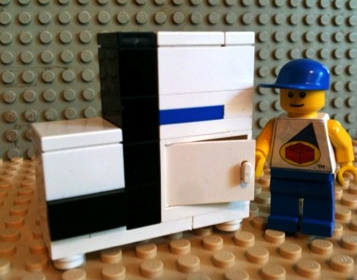
\includegraphics[width=0.35\linewidth,transparent]{hiseq.png}
  \end{center}
\end{frame}

\section{Sample processing}

\frame{
  \frametitle{Genome of the Netherlands}
  \tableofcontents[currentsection]
}

\begin{frame}
  \frametitle{Raw sequencing data}

  \vspace{\baselineskip}

  \begin{itemize}
    \item 750 samples
    \item 100GB per sample
    \item 75TB of FASTQ files
  \end{itemize}

  \vspace{\baselineskip}

\begin{center}
{\renewcommand{\arraystretch}{0.6}
\renewcommand{\tabcolsep}{10pt}
\begin{tabular}{p{200pt} r@{.}l}
  Human genome & 0&001\\
  Average PC & 0&1\\
  GoNL & \multicolumn{1}{r@{\phantom{.}}}{75}&\\
  3D effects rendering for Avatar & \multicolumn{1}{r@{\phantom{.}}}{1,000}&\\
  Google processes per day & \multicolumn{1}{r@{\phantom{.}}}{24,000}&
\end{tabular}}
\end{center}
\end{frame}

\begin{frame}
  \frametitle{Pipeline}

  \vspace{\baselineskip}

  Developed at UMCG

  \vspace{\baselineskip}

  \begin{itemize}
    \item Alignment
    \item SNP calling
    \item Based on Broad (GATK) pipeline
  \end{itemize}

  \vspace{\baselineskip}

  \url{http://www.bbmriwiki.nl/wiki/SnpCallingPipeline}
\end{frame}

\begin{frame}
  \frametitle{Hardware}

  \vspace{\baselineskip}

  \begin{itemize}
    \item Millipede cluster (RUG)
    \item Also: AMC (grid), UU, EMC
    \item Done in a month from now
  \end{itemize}

  % UMCG: ~250 lanes per week
  % UU and EMC: ~13 lanes per week
  % EMC: 0 lanes per week

  \vspace{0.5\baselineskip}

  \begin{center}
    
\includegraphics[width=0.45\linewidth,transparent]{millipedes.jpg}
  \end{center}
\end{frame}

\section{Quality control}

\frame{
  \frametitle{Genome of the Netherlands}
  \tableofcontents[currentsection]
}

\begin{frame}
  \frametitle{Phases}

  \vspace{\baselineskip}

  \begin{itemize}
    \item Pre-alignment
    \item Alignment
    \item Variant calling
  \end{itemize}
\end{frame}

\begin{frame}
  \frametitle{Pre-alignment}

  \vspace{\baselineskip}

  \begin{itemize}
    %\item Duplicate input checking
    \item FASTQ quality scores
    \item GC content
    \item N-content
    \item Read length distribution
    \item Over-representation of reads
  \end{itemize}
\end{frame}

\begin{frame}
  \frametitle{Alignment}

  \vspace{\baselineskip}

  \begin{itemize}
    \item Percentage aligned
    \item Insert size distribution
    \item Coverage distribution (X/Y/autosomal)
    \item Mapping quality distribution
  \end{itemize}
  % todo: picture of aligned reads?
\end{frame}

\begin{frame}
  \frametitle{Variant calling}

  \vspace{\baselineskip}

  \begin{itemize}
    \item Transition / transversion rate
    \item Mutation rate Y/mtDNA/autosomal
    \item Distribution of SNPs found in dnSNP
    \item Indel / substitution rate
  \end{itemize}
\end{frame}

\begin{frame}
  \frametitle{Pipeline concordance}

  \vspace{\baselineskip}

  Comparison of pipelines on alignment and variant calling

  \vspace{\baselineskip}

  \begin{itemize}
    \item SOAP pipeline (BGI)
    \item Broad pipeline (UMCG)
    \item GAPSS3 pipeline (LUMC)
    \item (Immuno-chip)
  \end{itemize}
\end{frame}

\begin{frame}
  \frametitle{SNP call concordance}

  \vspace{\baselineskip}

  Laurent Francioli:
  \begin{itemize}
    \item 50 samples
    \item SOAP (BGI) versus Broad (UMCG)
    \item Site and allele concordance
  \end{itemize}
\end{frame}

{
  \setbeamercolor{background canvas}{bg=}
  \usebackgroundtemplate{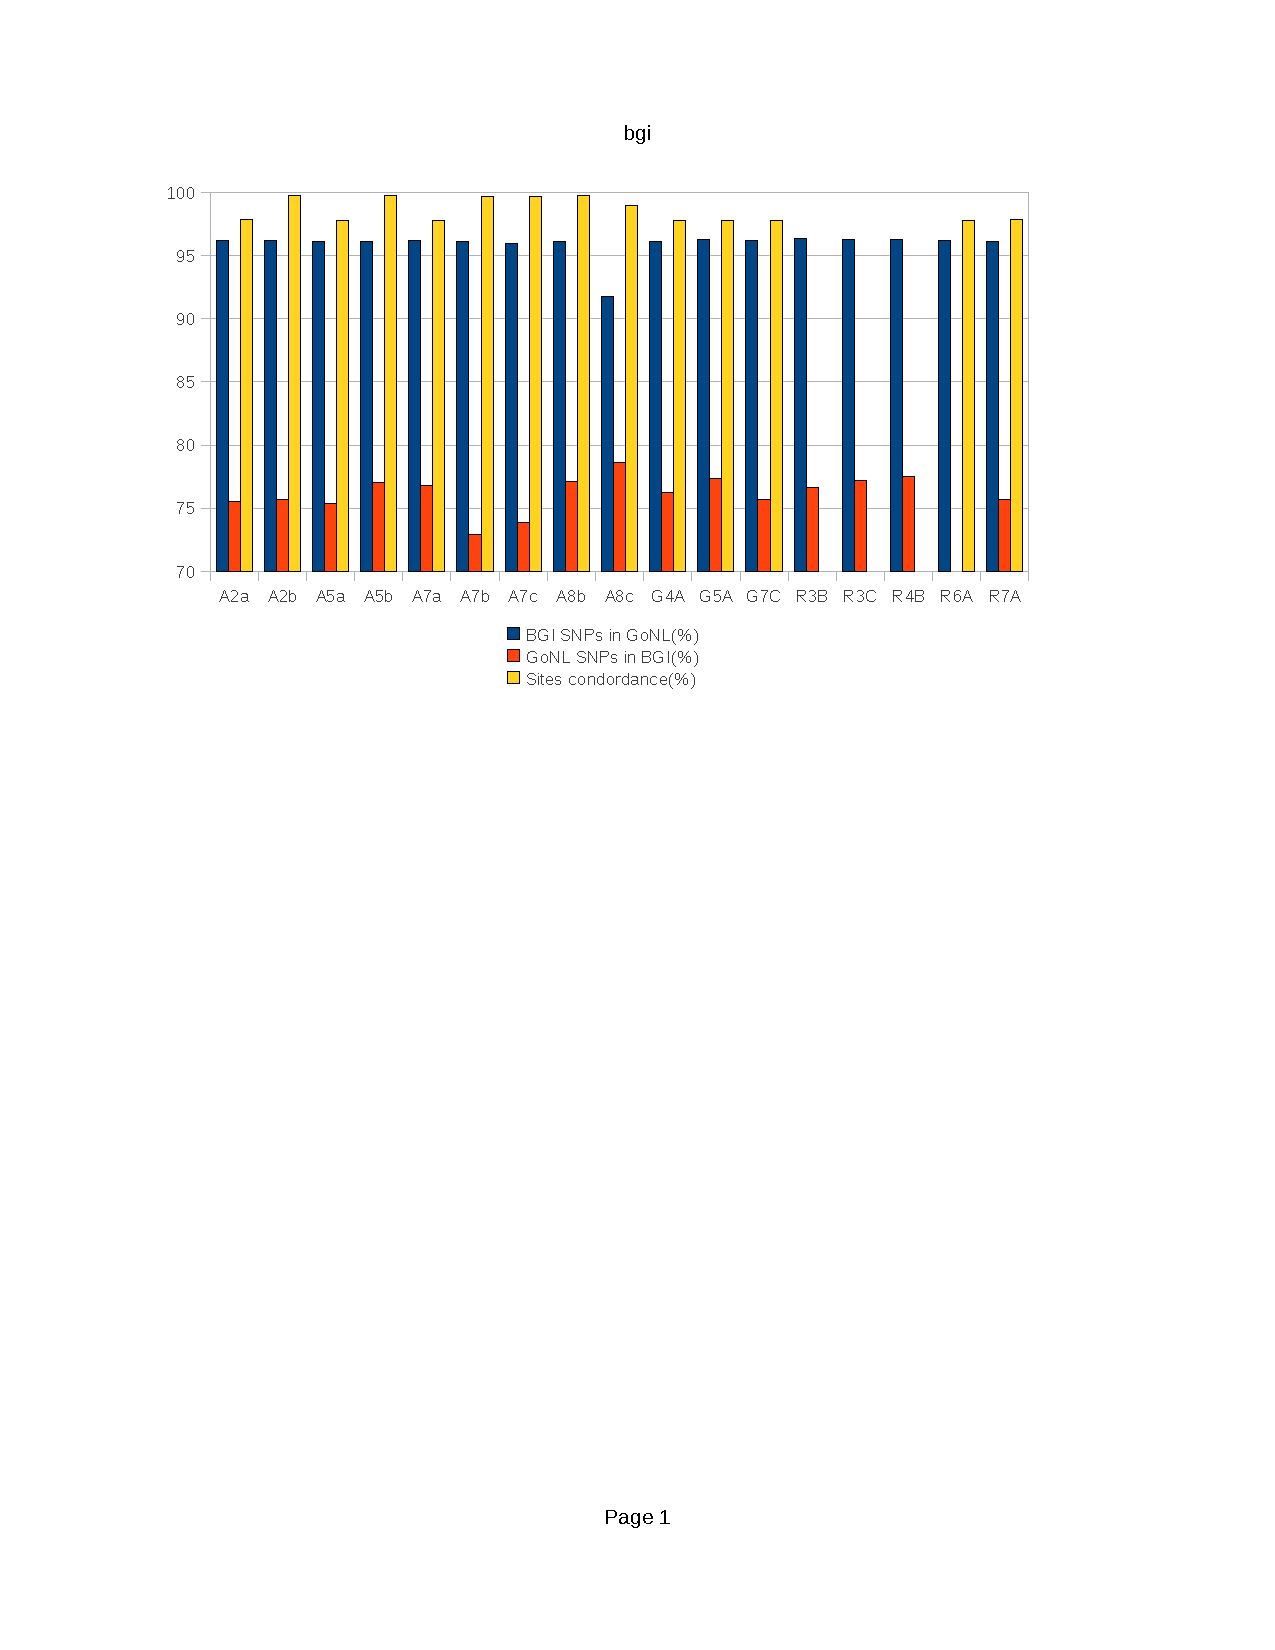
\includegraphics[width=\paperwidth,keepaspectratio=true,clip=true,trim=2cm 10cm 3cm 0]{bgi-concordance.pdf}}
  \frame{}
}

\begin{frame}
  \frametitle{SNP call concordance}

  \vspace{\baselineskip}

  Process 9 samples with GAPSS3 (LUMC)

  \vspace{\baselineskip}

\begin{center}
{\renewcommand{\arraystretch}{1.0}
\renewcommand{\tabcolsep}{10pt}
\begin{tabular}{p{140pt} r}
Pipeline & A4a SNPs\\
\hline
SOAP (BGI) & 3,204,825\\
Broad (UMCG) & 3,769,099\\
GAPSS3 (LUMC) & 3,374,486\\
GAPSS3 filtered & 2,459,515
\end{tabular}}
\end{center}

\end{frame}

{
  \setbeamercolor{background canvas}{bg=}
  \usebackgroundtemplate{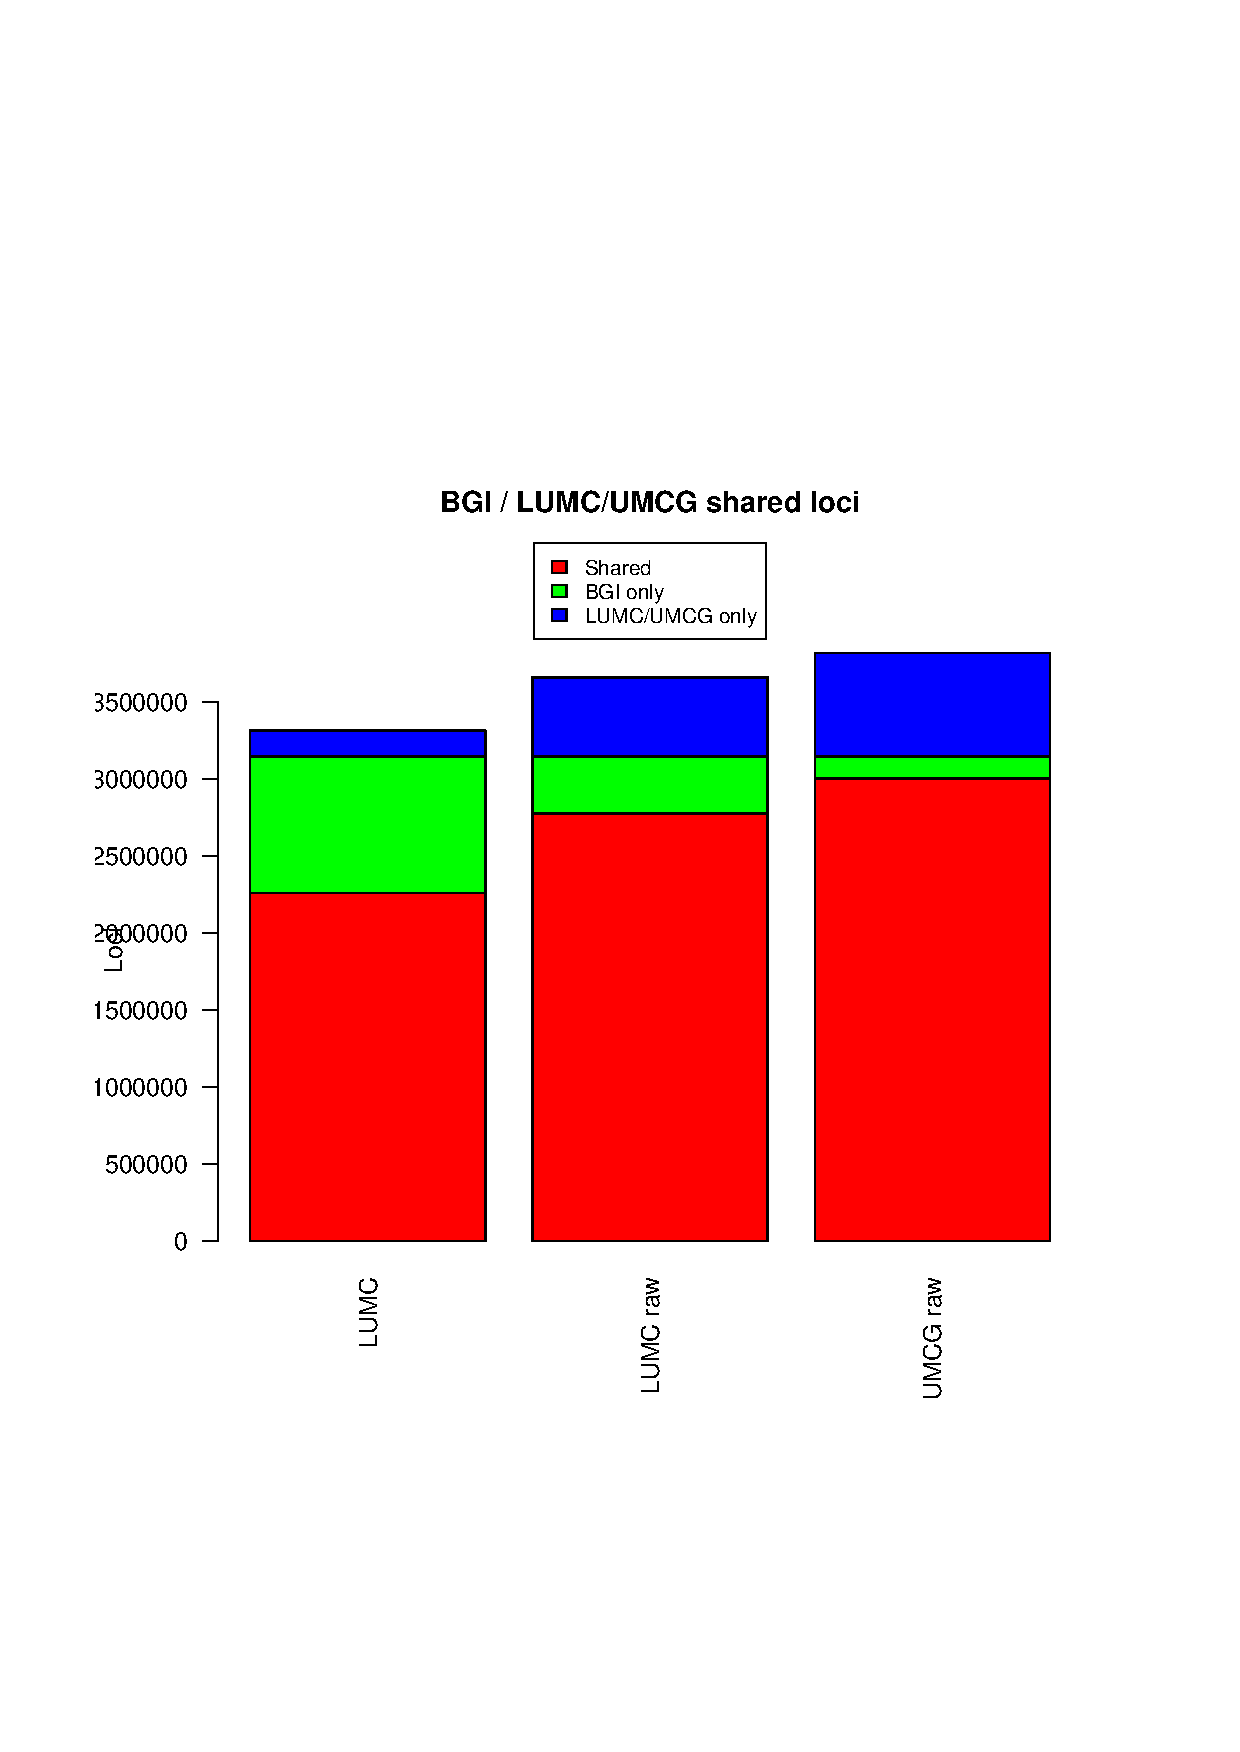
\includegraphics[width=0.65\paperwidth,keepaspectratio=true,clip=true,trim=0 3cm 3cm 5cm]{lumc-comparison.pdf}}
  \frame{}
}

{
  \setbeamercolor{background canvas}{bg=}
  \usebackgroundtemplate{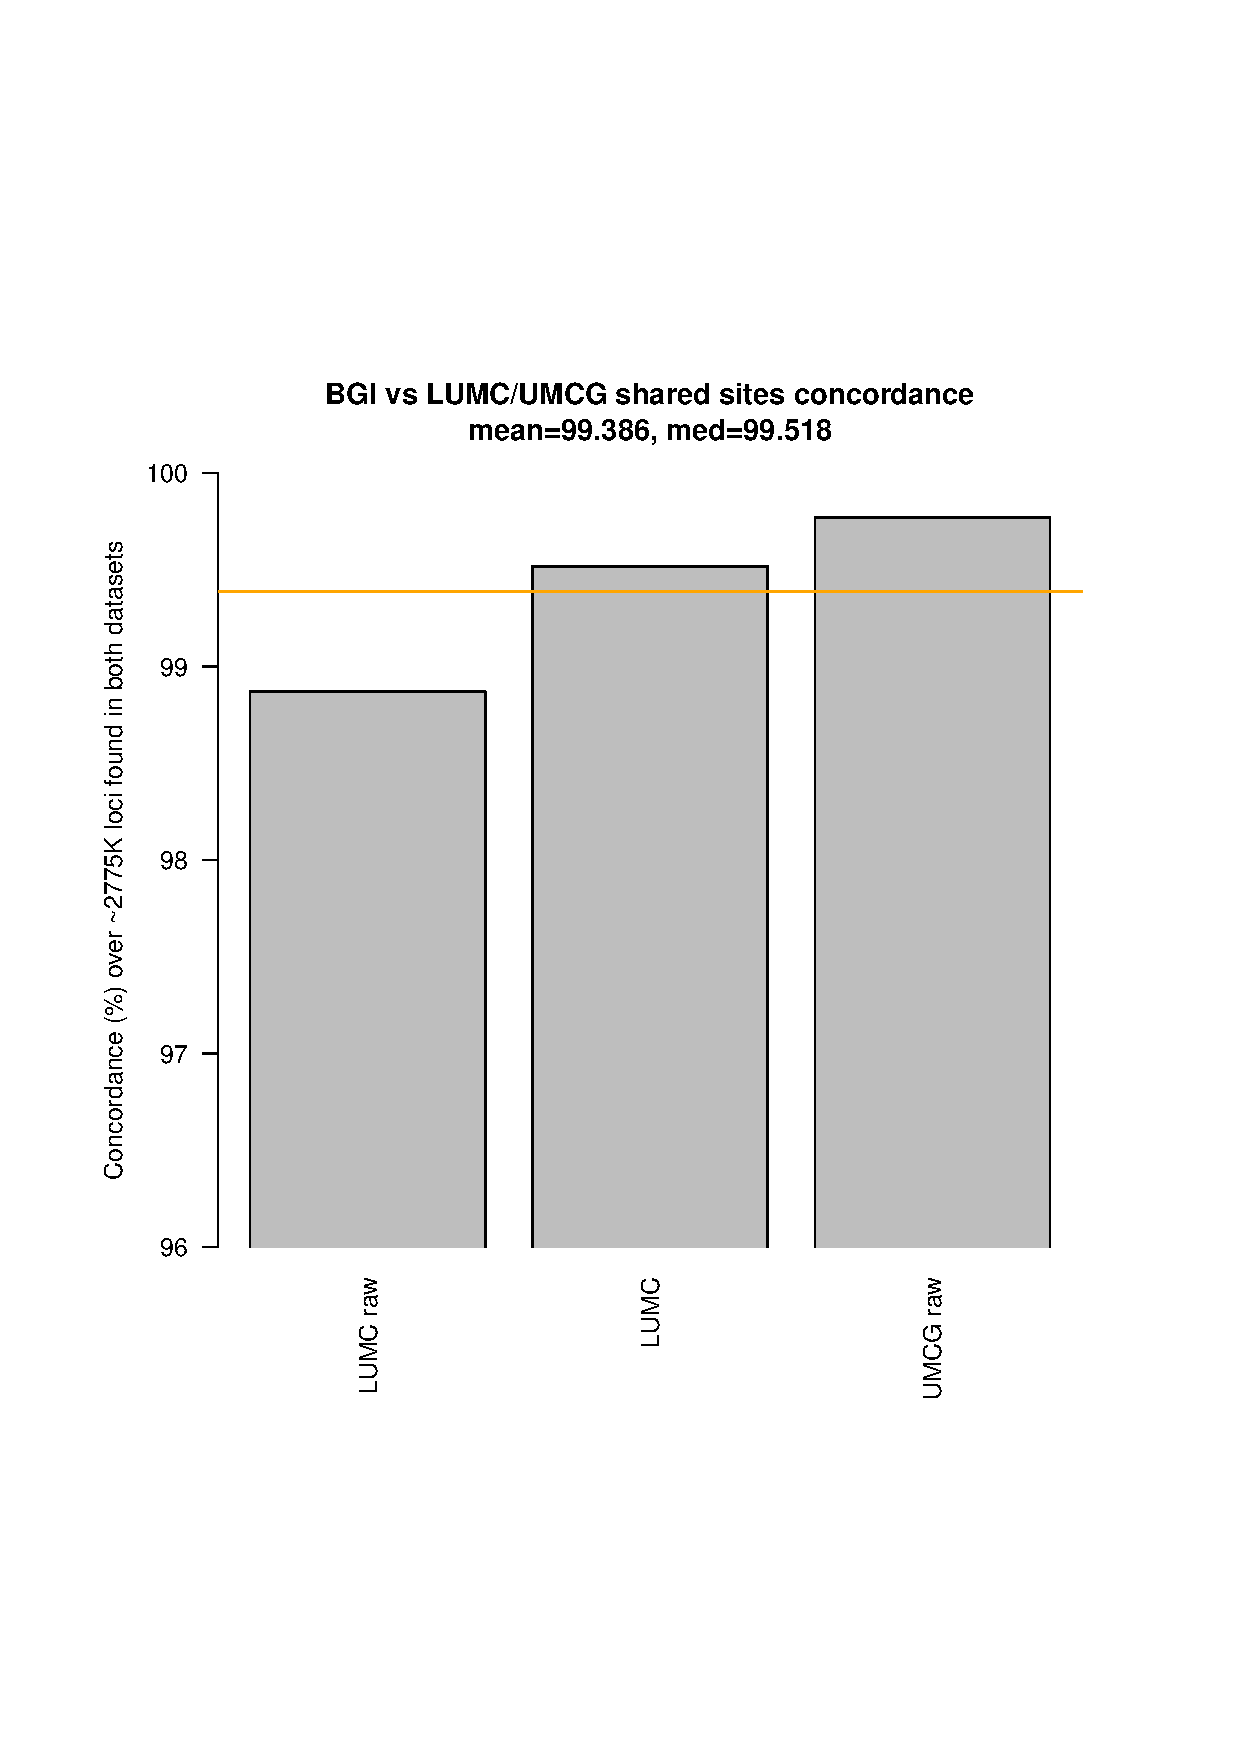
\includegraphics[width=0.65\paperwidth,keepaspectratio=true,clip=true,trim=0 3cm 3cm 5cm]{lumc-concordance.pdf}}
  \frame{}
}

\section{Mitochondrial DNA}

\frame{
  \frametitle{Genome of the Netherlands}
  \tableofcontents[currentsection]
}

\begin{frame}
  \frametitle{Mitochondria}

  \vspace{\baselineskip}

  50 to hundreds per cell

  \vspace{0.5\baselineskip}

  DNA:
  \begin{itemize}
    \item Circular, 16kbp
    \item 5--10 copies per mt
    \item Maternally inherited
  \end{itemize}

  \vspace{-\baselineskip}

  %\begin{center}
  \hspace{0.6\linewidth}
\includegraphics[width=0.3\linewidth,transparent]{mitochondrion.png}
  %\end{center}
\end{frame}

\begin{frame}
  \frametitle{Analysis}

  \vspace{\baselineskip}

  \begin{enumerate}
    \item Haplogroep info
    \item Heteroplasmy/sequence artefact herkenning
    \item DE-NOVO herkenning
  \end{enumerate}
\end{frame}

\section{Y chromosome}

\frame{
  \frametitle{Genome of the Netherlands}
  \tableofcontents[currentsection]
}

\begin{frame}
  \frametitle{Analysis}

  \vspace{\baselineskip}

  \begin{enumerate}
    \item Focus on 150,000bp non-repetitive part
    \item Compare to Y-tree and look voor DE-NOVO's
    \item Focus on Chris Tyler's Y-part
    \item Look at female reads mapping to Y
  \end{enumerate}
\end{frame}

\section{Questions?}

\frame{
  \frametitle{Genome of the Netherlands}
  \tableofcontents[currentsection]
}

\lastpagetemplate
\begin{frame}
  \begin{center}
    Acknowledgements:
    \bigskip
    \bigskip
    Jeroen Laros
  \end{center}
\end{frame}

\end{document}
